\documentclass[9pt]{beamer}
\usetheme[progressbar=frametitle]{metropolis}

% Packages
\usepackage{appendixnumberbeamer}
\usepackage{booktabs}
\usepackage[scale=2]{ccicons}
\usepackage{graphicx}
\usepackage{amsmath}
\usepackage[font=tiny,skip=2pt]{caption}
\usepackage{subcaption}
\usepackage{xcolor}

\usepackage{siunitx}
\sisetup{
  detect-weight=true,
  detect-family=true,
  table-number-alignment = center,
  table-format=3.6,
  table-space-text-post = **
}

% Customize caption and table spacing for Beamer slides
\makeatletter
\AtBeginDocument{%
  \setbeamerfont{caption}{size=\tiny}
  \setbeamerfont{caption name}{size=\tiny}
  \setlength{\abovecaptionskip}{1pt}
  \setlength{\belowcaptionskip}{1pt}
  \renewenvironment{table}[1][]{%
    \def\@captype{table}%
    \par\vspace{0.15em}%
    \centering
  }{%
    \par\vspace{0.15em}%
  }%
}
\makeatother

% Title Info
\title{\Huge Modelling \& Forecasting\\Spanish Real GDP Growth}
\subtitle{Econometrics 20203 - Problem Set 2 (Quarterly Data)}
\author{Stefano Graziosi - 3174891 \\
        Gabriele Biroli - 3165990 \\
        Luca Gritti - 3037416
        }
\institute{MSc Economic and Social Sciences, Università Bocconi}
\date{\today}

\begin{document}

\maketitle

% ============================================================
% SLIDE 1: Question, Data, and Forecasting Design
% ============================================================
\begin{frame}{Question, data, and forecasting design}
\label{slide:setup}
\footnotesize

\begin{columns}[T]
\begin{column}{0.5\textwidth}
\begin{block}{Data}
\begin{itemize}\setlength{\itemsep}{1pt}
  \item \textbf{Country:} Spain
  \item \textbf{Quarterly sample:} 2001Q1--2025Q4 (100 observations).
  \item \textbf{Target:} $g_t$, real GDP growth (YoY \%).
  \item \textbf{Predictors:} HICP inflation $\pi_t$ (YoY \%) and short-term interest rate $i_t$ (3-month EURIBOR, \%).
  \item \textbf{Source:} Barigozzi, Lissona \& Tonni (2025); short rate (3-month EURIBOR) from the ECB Data Portal.
\end{itemize}
\end{block}
\end{column}

\begin{column}{0.5\textwidth}
\begin{block}{Specifications for the forecasting}
\begin{itemize}\setlength{\itemsep}{1pt}
  \item \textbf{Evaluation window:} 2016Q1--2025Q4 (10 years, 40 quarterly forecasts).
  \item \textbf{Horizon:} 1-quarter-ahead point forecasts.
  \item \textbf{Estimation:} recursive expanding window.
  \item \textbf{Software:} R; OLS and Bayesian VAR estimation.
\end{itemize}
\end{block}
\end{column}
\end{columns}

\vspace{0.15cm}
The selected variables span the canonical New-Keynesian system: aggregate demand (GDP), price stability (inflation), and the monetary-policy stance (short-term interest rate).

\end{frame}


% ============================================================
% SLIDE 2: Spain's GDP Growth History & Phases
% ============================================================
\begin{frame}{Descriptive macro picture}
\label{slide:history}
\begin{block}{}
\footnotesize
The quarterly series capture the major macroeconomic phases of the euro era:
\end{block}

\begin{columns}

  \begin{column}{0.55\textwidth}
    \centering
    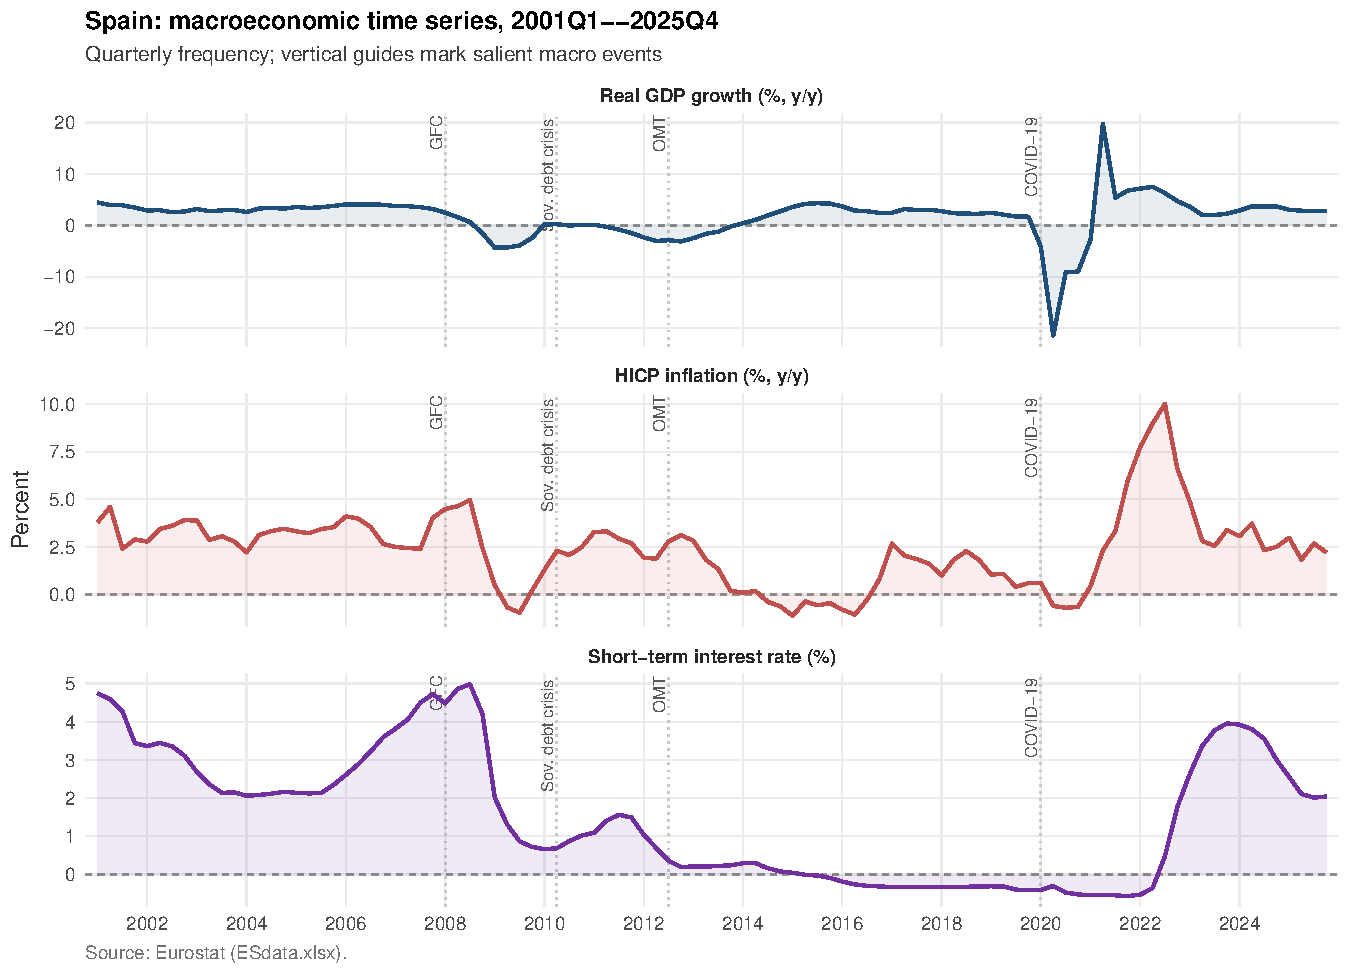
\includegraphics[width=\linewidth]{figures_q/descriptive_plots.pdf}
  \end{column}

  \begin{column}{0.45\textwidth}
    \scriptsize
    \begin{itemize}
      \item \textbf{2001--2007:} The pre-GFC expansion features robust, steady growth (often around 3--4 percent y/y), fueled by the construction boom and cheap credit post-euro adoption.
      \item \textbf{2008--2013:} A severe double-dip recession. The initial Global Financial Crisis (2008--2009) is followed by the euro-area sovereign-debt crisis (2011--2013), pushing growth deeply negative.
      \item \textbf{2014--2025:} The recovery is interrupted by the extreme COVID-19 shock of 2020Q2 (--21.5 percent y/y). The subsequent rebound is accompanied by the post-2021 energy-driven inflation spike and the resulting interest-rate tightening cycle, before normalising in 2024--25.
    \end{itemize}
  \end{column}

\end{columns}

\end{frame}


% ============================================================
% SLIDE 3: Descriptive Statistics
% ============================================================
\begin{frame}{Descriptive statistics: scale and distributions}
\label{slide:descriptive}

{\footnotesize
\setlength{\tabcolsep}{4pt}
\begin{table}

\caption{\label{tab:summary-stats}Summary statistics, 2001Q1--2025Q4 (quarterly)}
\centering
\begin{tabular}[t]{lrrrrrrrr}
\toprule
Variable & N & Mean & Std. dev. & Min & Median & Max & Skewness & Kurtosis\\
\midrule
GDP growth (\%) & 100 & 1.73 & 4.18 & -21.45 & 2.72 & 19.77 & -1.35 & 14.27\\
Inflation (\%) & 100 & 2.36 & 2.02 & -1.12 & 2.49 & 10.01 & 0.79 & 4.98\\
ST rate (\%) & 100 & 1.52 & 1.72 & -0.57 & 1.20 & 4.98 & 0.41 & 1.80\\
\bottomrule
\end{tabular}
\end{table}

}

{\footnotesize
\begin{itemize}
    \item \textbf{GDP growth} exhibits severe left-tail behaviour (negative skewness and kurtosis well above the Gaussian value of three), driven largely by the massive COVID-19 contraction of 2020Q2 (--21.5\%) and the GFC. The overall mean is pulled down compared to the pre-2008 trend.

    \item \textbf{Inflation} shows moderate right-skewness, mainly reflecting the intense, though brief, post-pandemic energy price shock. The 10.1\% peak contrasts with the mildly deflationary episodes of 2009 and 2014.

    \item \textbf{Short-term rate} (3-month EURIBOR) is mildly right-skewed and platykurtic. It traces the ECB policy cycle: a $\sim$5\% pre-GFC peak (2008), the near-zero and \emph{negative}-rate era of 2015--2022 (a --0.6\% trough in 2021), and the steep 2022--23 hiking cycle.
\end{itemize}
}

\end{frame}


% ============================================================
% SLIDE 4: Marginal Distributions & Bivariate Structure
% ============================================================
\begin{frame}{Marginal Distributions \& Bivariate Structure}
\label{slide:distributions}
\footnotesize
\begin{block}{}
\begin{columns}
  \begin{column}{0.5\textwidth}
    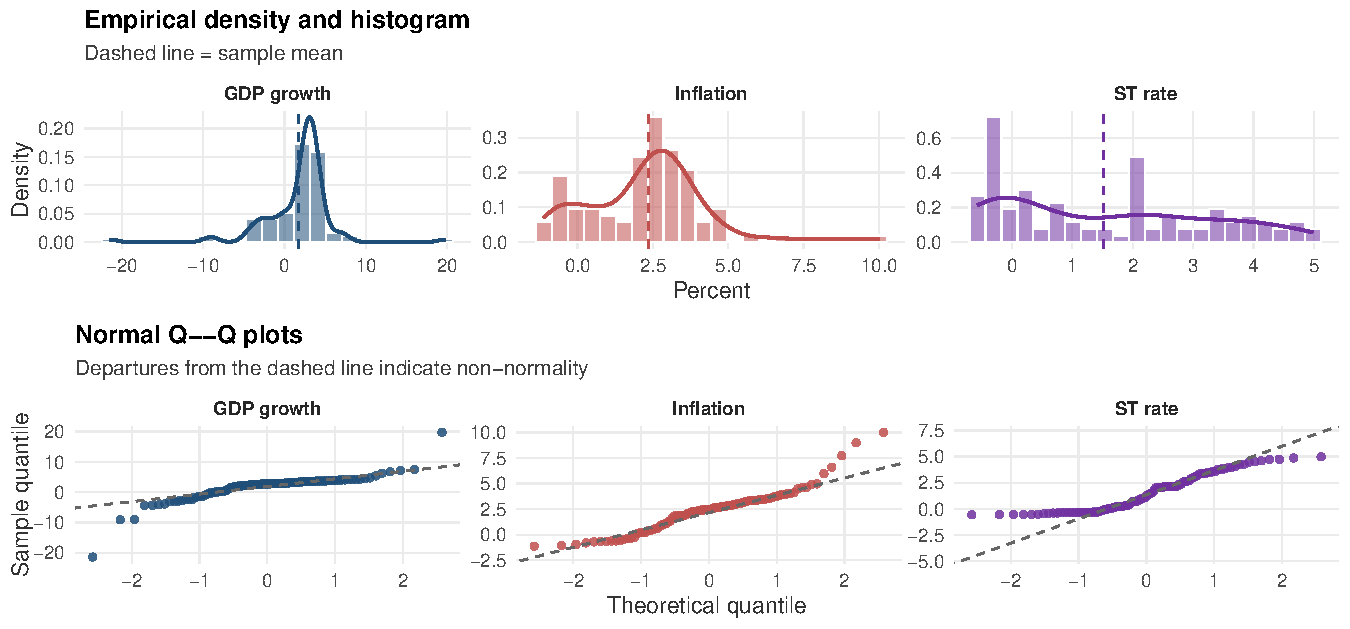
\includegraphics[width=\linewidth]{figures_q/distribution_plots.pdf}
  \end{column}
  \begin{column}{0.5\textwidth}
    The histograms confirm the asymmetries: GDP growth has a very long left tail (COVID and GFC), while inflation is slightly right-skewed. The Q–Q plots confirm systematic deviations from normality in the tails. As we will see in Slide~\ref{slide:diagnostics}, this heavy-tailed behaviour—particularly from COVID—translates into rejections of normality for the model residuals.
  \end{column}
\end{columns}
\end{block}

\vspace{0.3cm}

\begin{block}{}
\begin{columns}
  \begin{column}{0.5\textwidth}
    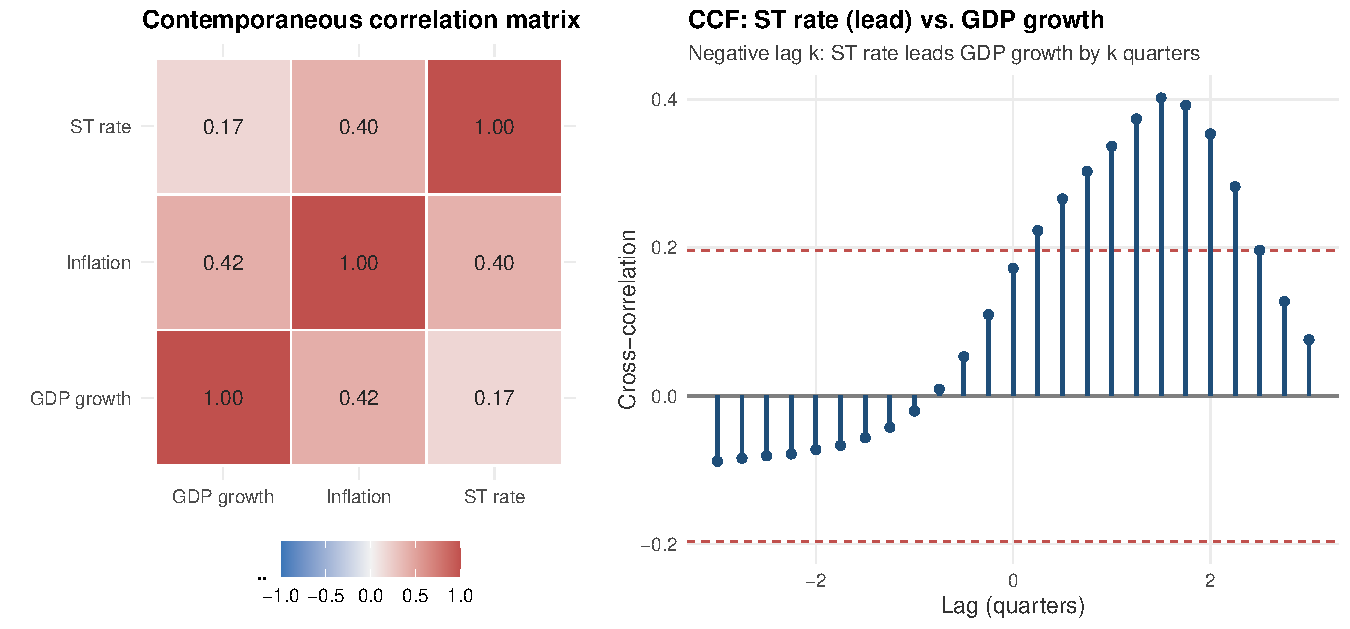
\includegraphics[width=\linewidth]{figures_q/scatter_corr.pdf}
  \end{column}
  \begin{column}{0.5\textwidth}
    GDP growth and the short-term rate are only weakly correlated contemporaneously, while inflation and the short-term rate are positively correlated ($\approx 0.4$), consistent with an ECB monetary-policy reaction. The cross-correlation function shows that growth and inflation tend to \emph{lead} the short rate, identifying it as a cyclically reactive policy variable rather than a leading indicator of activity.
  \end{column}
\end{columns}
\end{block}
\end{frame}


% ============================================================
% SLIDE 5: Rolling-Window Moments & Autocorrelation Structure
% ============================================================
\begin{frame}{Persistence in GDP growth \& Rolling Moments}
\label{slide:rolling}
\footnotesize
\begin{block}{}
\begin{columns}
  \begin{column}{0.5\textwidth}
    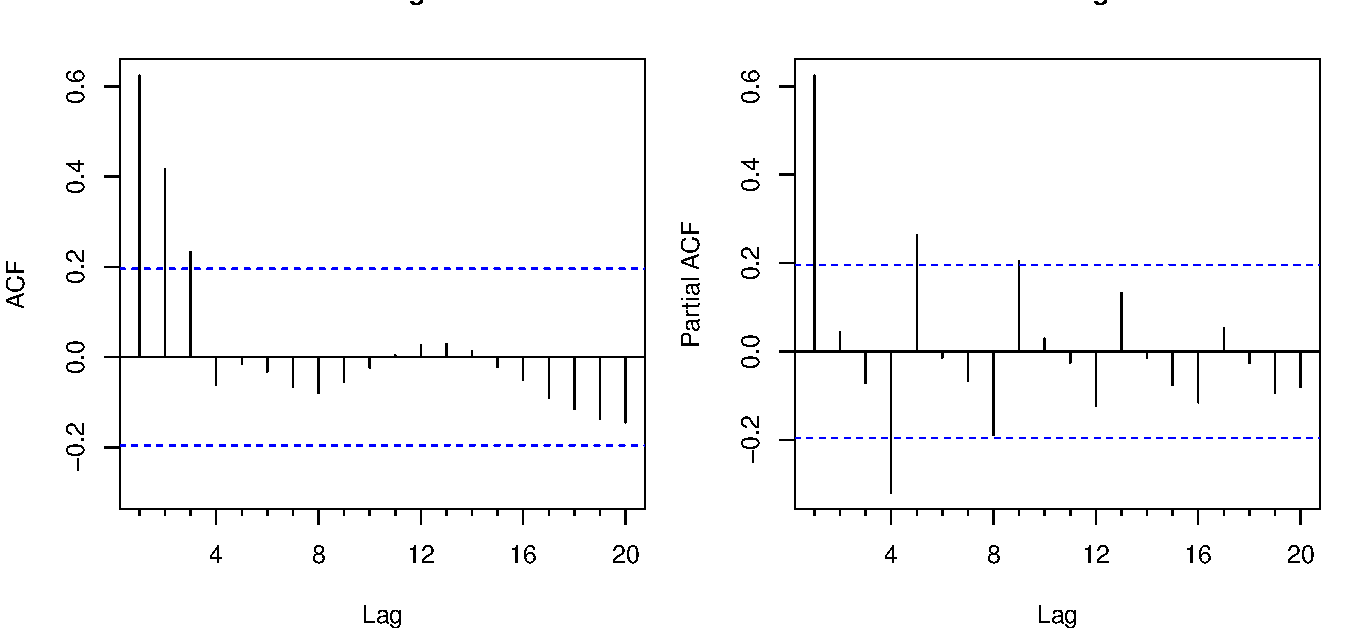
\includegraphics[width=\linewidth]{figures_q/acf_pacf.pdf}
  \end{column}
  \begin{column}{0.5\textwidth}
    The ACF decays slowly from a high first-order coefficient, reflecting the strong persistence of year-on-year quarterly growth rates (which mechanically overlap by three quarters). The PACF displays significant spikes at the first few lags, consistent with a low-order autoregressive process. This motivates our AR(p) and ARIMA models.
  \end{column}
\end{columns}
\end{block}

\vspace{0.4cm}

\begin{block}{}
\begin{columns}
  \begin{column}{0.5\textwidth}
    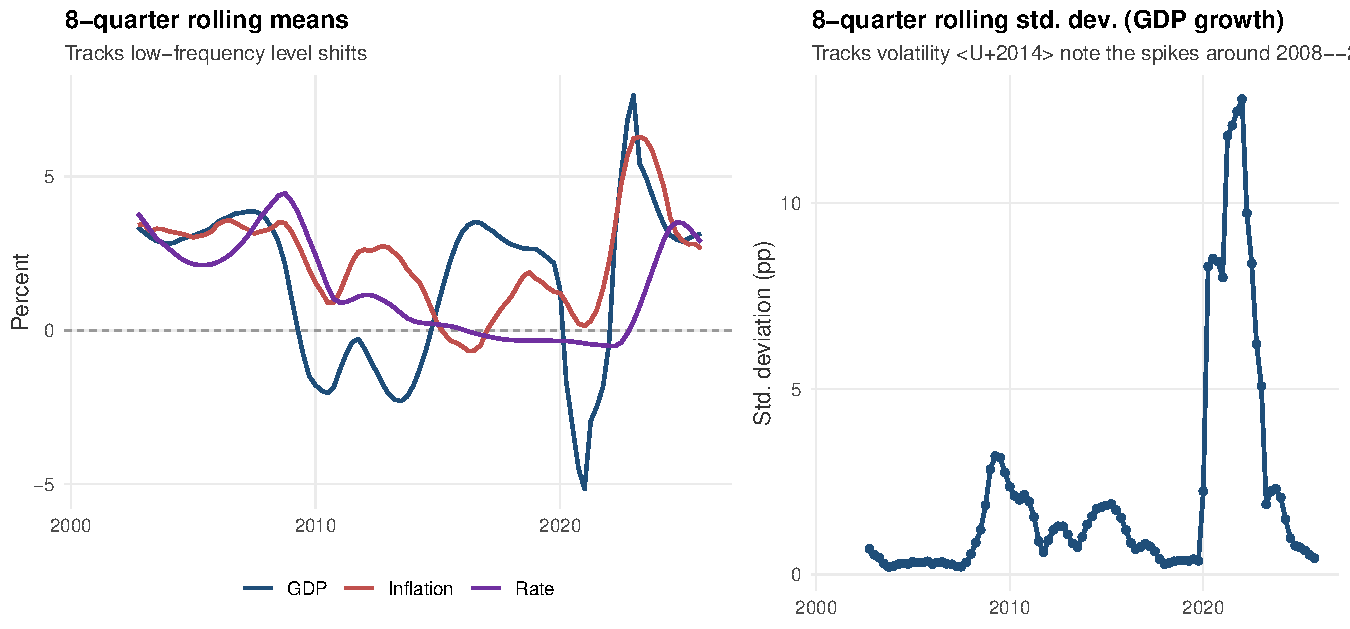
\includegraphics[width=\linewidth]{figures_q/rolling_stats.pdf}
  \end{column}
  \begin{column}{0.5\textwidth}
    Rolling means (8-quarter window) highlight the ECB policy cycle in the short-term rate---cuts to near-zero and below during 2012--2021, then the sharp 2022--23 tightening---and the dramatic plunge in average growth during the GFC and COVID-19. Rolling standard deviation spikes precisely during these crisis episodes, warning of time-varying volatility and potential structural breaks.
  \end{column}
\end{columns}
\end{block}
\end{frame}


% ============================================================
% SLIDE 6: Stationarity Tests
% ============================================================
\begin{frame}{(Preliminary) Diagnostic Checks: Stationarity}
\label{slide:stationarity}
\footnotesize
Table~\ref{tab:tbl-unit-roots-q} reports ADF (null: unit root) and KPSS (null: level stationarity) tests. We combine the two so that conclusions agree only when both procedures reject in the appropriate direction.

{\footnotesize
\setlength{\tabcolsep}{5pt}
\begin{table}

\caption{\label{tab:tbl-unit-roots-q}Unit-root tests, 2001Q1--2025Q4 (quarterly)}
\centering
\begin{tabular}[t]{lrrrr}
\toprule
Variable & ADF stat & ADF p-value & KPSS stat & KPSS p-value\\
\midrule
GDP growth & -3.360 & 0.065 & 0.127 & 0.10\\
Inflation & -2.358 & 0.428 & 0.228 & 0.10\\
ST rate & -2.523 & 0.360 & 0.757 & 0.01\\
\bottomrule
\end{tabular}
\end{table}

}

\footnotesize
\begin{itemize}
  \item \textbf{GDP growth is borderline stationary.} ADF rejects the unit root only at the 10\% level (p $=$ 0.07), while KPSS does \emph{not} reject level stationarity (p $>$ 0.10); together with its evident mean reversion this supports treating $\Delta y_t$ as $I(0)$, a standard macroeconometric choice.

  \item \textbf{Inflation and the short-term rate} are highly persistent: ADF fails to reject a unit root for both, and KPSS strongly rejects stationarity for the short-term rate. Following the macroeconomic literature, we keep the variables in \textit{levels} rather than differencing them, since (a) the Bayesian VAR's Minnesota prior shrinks coefficients toward a random walk and accommodates persistent regressors, and (b) cointegration with growth is plausible and economically meaningful.
\end{itemize}

\end{frame}


% ============================================================
% SLIDE 7: Cointegration Analysis
% ============================================================
\begin{frame}{(Preliminary) Diagnostic Checks: Cointegration}
\label{slide:cointegration}
\footnotesize

\begin{columns}

  \begin{column}{0.54\textwidth}
    {\fontsize{5.5}{6}\selectfont
    \setlength{\tabcolsep}{2.5pt}
    \setlength{\abovecaptionskip}{2pt}
    \setlength{\belowcaptionskip}{1pt}
    \begin{table}

\caption{\label{tab:engle-granger}Engle--Granger residual-based cointegration test (quarterly)}
\centering
\begin{tabular}[t]{lr}
\toprule
Statistic & Value\\
\midrule
ADF (no constant) on EG residuals & -3.34\\
1\% critical value & -2.60\\
5\% critical value & -1.95\\
10\% critical value & -1.61\\
\bottomrule
\end{tabular}
\end{table}

    \vspace{0.1cm}
    \begin{table}

\caption{\label{tab:johansen}Johansen Trace test (no constant, no trend, K = 2) -- quarterly}
\centering
\begin{tabular}[t]{lrrrr}
\toprule
H0: rank <= r & Trace stat & 10\% & 5\% & 1\%\\
\midrule
r <= 2 & 8.259 & 6.50 & 8.18 & 11.65\\
r <= 1 & 25.308 & 15.66 & 17.95 & 23.52\\
r <= 0 & 47.042 & 28.71 & 31.52 & 37.22\\
\bottomrule
\end{tabular}
\end{table}

    \vspace{0.1cm}
    \begin{table}

\caption{\label{tab:vecm-loadings}Loading (adjustment) matrix $\alpha$ --- rows: equation, columns: ECT}
\centering
\begin{tabular}[t]{lrr}
\toprule
  & ECT1 & ECT2\\
\midrule
GDP growth & -0.377 & -0.065\\
Inflation & 0.043 & -0.183\\
ST rate & 0.006 & 0.040\\
\bottomrule
\end{tabular}
\end{table}

    }
  \end{column}

  \begin{column}{0.46\textwidth}
    \footnotesize
    \begin{itemize}\setlength{\itemsep}{2pt}\setlength{\parskip}{0pt}
      \item The \textbf{Engle--Granger} test on the static regression residuals provides single-equation evidence. 
      \item The \textbf{Johansen Trace} test rejects every reduced rank at the 5\% level (full rank), pointing to a (near-)stationary system rather than reduced-rank cointegration; we therefore rely on the level VAR/BVAR rather than a VECM.
      \item Given the assignment's explicit focus on level VAR and BVAR benchmarks, and the potential rank fragility in finite samples of 100 observations, we proceed with the unrestricted level VAR and its Minnesota-shrinkage counterpart, which are robust to cointegration without explicitly imposing the VECM constraints.
    \end{itemize}
  \end{column}

\end{columns}

\end{frame}


% ============================================================
% SLIDE 8: Model Specifications
% ============================================================
\subsection{Model Specification}
\begin{frame}{Model specification strategy}
\label{slide:models}
\small

\begin{columns}
  \begin{column}{0.54\textwidth}
    {\fontsize{5}{5.5}\selectfont
    \setlength{\tabcolsep}{2.5pt}
    \setlength{\abovecaptionskip}{1pt}
    \setlength{\belowcaptionskip}{1pt}
    \begin{table}

\caption{\label{tab:ar-arima-models}AR(p) information criteria (quarterly)}
\centering
\begin{tabular}[t]{rrr}
\toprule
p & AIC & BIC\\
\midrule
0 & 572.65 & 577.86\\
1 & 525.48 & 533.29\\
2 & 527.28 & 537.70\\
3 & 528.81 & 541.84\\
4 & 520.43 & 536.07\\
\addlinespace
5 & 515.44 & 533.68\\
\bottomrule
\end{tabular}
\end{table}

    \vspace{0.1cm}
    \begin{table}

\caption{\label{tab:ar2-coef}AR(2): coefficient estimates (quarterly)}
\centering
\begin{tabular}[t]{lrr}
\toprule
term & estimate & std.error\\
\midrule
ar1 & 0.593 & 0.099\\
ar2 & 0.044 & 0.099\\
intercept & 1.797 & 0.877\\
\bottomrule
\end{tabular}
\end{table}

    \vspace{0.1cm}
    \begin{table}

\caption{\label{tab:var-summary}VAR(2): equation for GDP growth (quarterly)}
\centering
\begin{tabular}[t]{lrrrr}
\toprule
term & estimate & std.error & statistic & p.value\\
\midrule
GDP\_Growth.l1 & 0.545 & 0.110 & 4.962 & 0.000\\
Inflation.l1 & 0.451 & 0.400 & 1.128 & 0.262\\
Interest\_Rate.l1 & 0.998 & 1.050 & 0.951 & 0.344\\
GDP\_Growth.l2 & 0.059 & 0.109 & 0.537 & 0.593\\
Inflation.l2 & -0.531 & 0.404 & -1.315 & 0.192\\
\addlinespace
Interest\_Rate.l2 & -0.910 & 0.986 & -0.923 & 0.359\\
const & 0.746 & 0.568 & 1.315 & 0.192\\
\bottomrule
\end{tabular}
\end{table}

    }
  \end{column}

  \begin{column}{0.46\textwidth}
    \footnotesize
    Five models are evaluated, balancing univariate persistence against multivariate macro-financial linkages:
    \begin{itemize}\setlength{\itemsep}{3pt}\setlength{\parskip}{0pt}
      \item The univariate criteria inform the choice of the \textbf{ARIMA (BIC)} baseline. The \textbf{AR(2)} is estimated to match the assignment specification, and its coefficient estimates confirm the high persistence.
      
      \item The multivariate criteria inform the lag selection for the VAR. To comply with the brief, we estimate a \textbf{VAR(2)}. With 100 observations and 21 parameters, the unrestricted VAR still pays a variance penalty.

      \item We treat the \textbf{BVAR(2)} as our preferred individual model on a priori grounds (favourable small-sample properties via Minnesota shrinkage).
      
      \item A \textbf{Combined} forecast (equal-weight average) provides simple insurance against picking the wrong single model.
    \end{itemize}
  \end{column}
\end{columns}

\end{frame}


% ============================================================
% SLIDE 9: Optimal Model Specification
% ============================================================
\begin{frame}{Why include a Bayesian VAR? (a-priori grounds)}
\label{slide:bvar}

\textbf{\footnotesize Why a Bayesian Vector Autoregression?}

\scriptsize
\begin{enumerate}
  \item \textbf{Captures simultaneous dynamics across the New-Keynesian triplet}\\
        The triple $(\Delta y,\,\pi,\,i)$ spans the canonical NK three-equation system. For Spain, the short-term rate (3-month EURIBOR) directly reflects the euro-area monetary-policy stance, so the model traces the transmission of monetary and financial conditions to domestic activity.

  \item \textbf{Bayesian shrinkage addresses the estimation variance problem}\\
        With 100 quarterly observations and 21 reduced-form parameters, the unrestricted OLS VAR faces over-fitting. The Minnesota prior anchors the posterior toward a parsimonious random-walk benchmark. It preserves the multivariate cross-equation information while regularising the coefficients.

  \item \textbf{Rich policy diagnostics}\\
        The BVAR delivers impulse responses and variance decompositions; here the GDP-growth response to a short-rate shock (Slide~\ref{slide:granger-irf}) is small and imprecisely estimated (its 90\% band spans zero), so no robust transmission is identified in this short sample.

  \item \textbf{Structural-break evidence motivates robust shrinkage, not splitting}\\
        As we will see in Slide~\ref{slide:breaks}, the structural-break tests strongly reject parameter constancy at the 2020 COVID shock. However, this is an exogenous outlier rather than a fundamental regime change. The Minnesota prior naturally absorbs such large innovations without requiring a fragile time-varying-parameter specification or splitting the sample.
\end{enumerate}

\end{frame}


% ============================================================
% SLIDE 10: Structural Stability — Tests, Interpretation & Visual Evidence
% ============================================================
\begin{frame}{Structural stability: breakpoint tests \& interpretation}
\label{slide:breaks}
\label{slide:breaks-interp}
\footnotesize

\begin{columns}[T]
  \begin{column}{0.5\textwidth}
    {\fontsize{5}{5.5}\selectfont
    \setlength{\tabcolsep}{1.5pt}
    \setlength{\abovecaptionskip}{2pt}
    \setlength{\belowcaptionskip}{1pt}
    \begin{table}

\caption{\label{tab:chow-tests}Chow F-tests for parameter constancy in the AR(2) for GDP growth (quarterly)}
\centering
\begin{tabular}[t]{lllrr}
\toprule
Test & Break date & Event & F-statistic & p-value\\
\midrule
CH1 & 2008Q1 & Global financial crisis & 0.383 & 0.766\\
CH2 & 2012Q3 & OMT/sovereign-debt crisis end & 1.648 & 0.184\\
CH3 & 2020Q2 & COVID-19 pandemic & 21.575 & 0.000\\
\bottomrule
\end{tabular}
\end{table}

    \vspace{0.05cm}
    \begin{table}

\caption{\label{tab:unknown-breaks}Unknown-date structural-break tests (quarterly)}
\centering
\begin{tabular}[t]{llll}
\toprule
Test & Statistic & Break date(s) & p-value\\
\midrule
Quandt--Andrews sup-F & 64.72 & 2020Q3 & 0.000\\
Bai--Perron (BIC-optimal m) & m = 2 & 2016Q4, 2020Q2 & <U+2014>\\
\bottomrule
\end{tabular}
\end{table}

    }
    \vspace{0.1cm}
    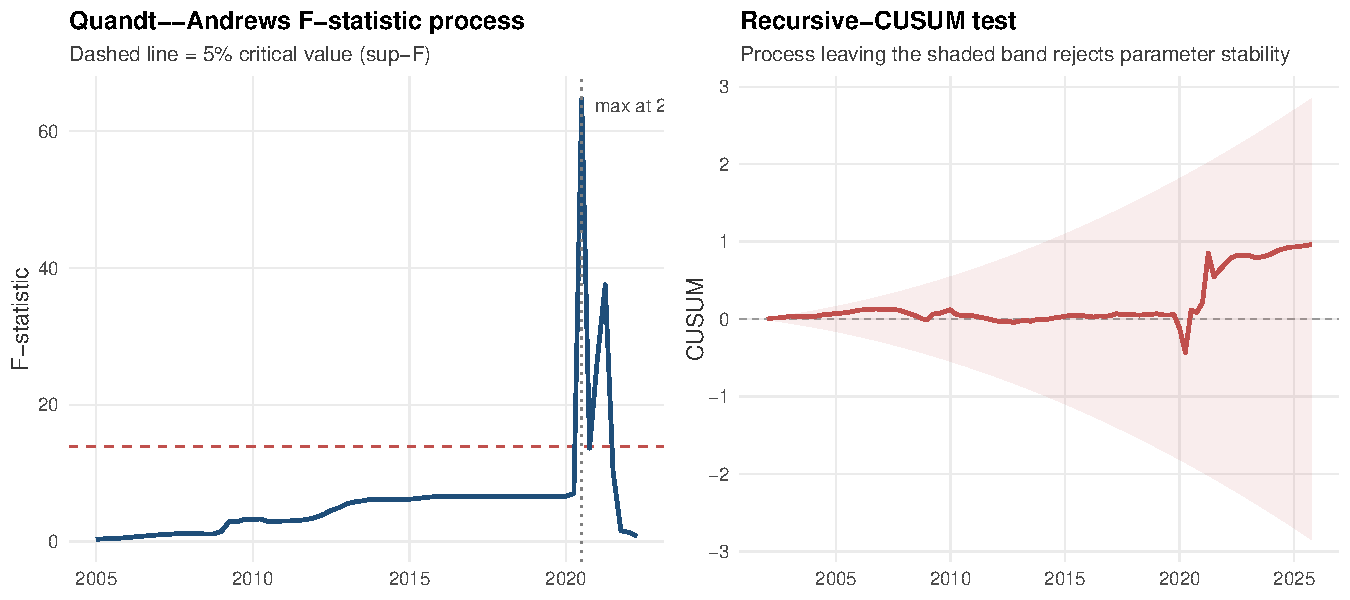
\includegraphics[width=\linewidth]{figures_q/qlr_cusum_plot.pdf}
  \end{column}

  \begin{column}{0.5\textwidth}
    \scriptsize
    \begin{itemize}\setlength{\itemsep}{1pt}\setlength{\parskip}{0pt}
      \item \textbf{CH1 (2008Q1):} GFC onset --- marginal-to-strong rejection as growth drops sharply.
      \item \textbf{CH2 (2012Q3):} Draghi's "whatever it takes" OMT, marking the end of the sovereign-debt phase.
      \item \textbf{CH3 (2020Q2):} decisively rejected --- the COVID contraction is a one-off of a different magnitude the linear AR(2) cannot accommodate.
      \item \textbf{Quandt--Andrews / Bai--Perron} unknown-break tests cluster instability around the GFC and COVID. The CUSUM drifts outside its bands and the QLR sup-$F$ peaks at 2020, confirming the COVID outlier.
    \end{itemize}
    \textbf{Two practical implications:}
    \begin{enumerate}\setlength{\itemsep}{1pt}\setlength{\parskip}{0pt}
      \item \textbf{Sample retention.} Pre-2020 dynamics are relatively stable (save GFC turbulence), so we keep the \textbf{full 2001Q1--2025Q4 sample}; splitting would discard vital history and cripple precision.
      \item \textbf{COVID treatment.} 2020 is a \textbf{one-off exogenous shock}, not a regime change --- no permanent dummy or TVP model. The BVAR's Minnesota prior shrinks robustly and prevents the outlier from distorting parameters.
    \end{enumerate}
  \end{column}
\end{columns}

\end{frame}


% ============================================================
% SLIDE 12: Diagnostic Checks
% ============================================================
\begin{frame}{Diagnostics for the VAR(2) baseline}
\label{slide:diagnostics}
\footnotesize

\begin{columns}
  \begin{column}{0.55\textwidth}
    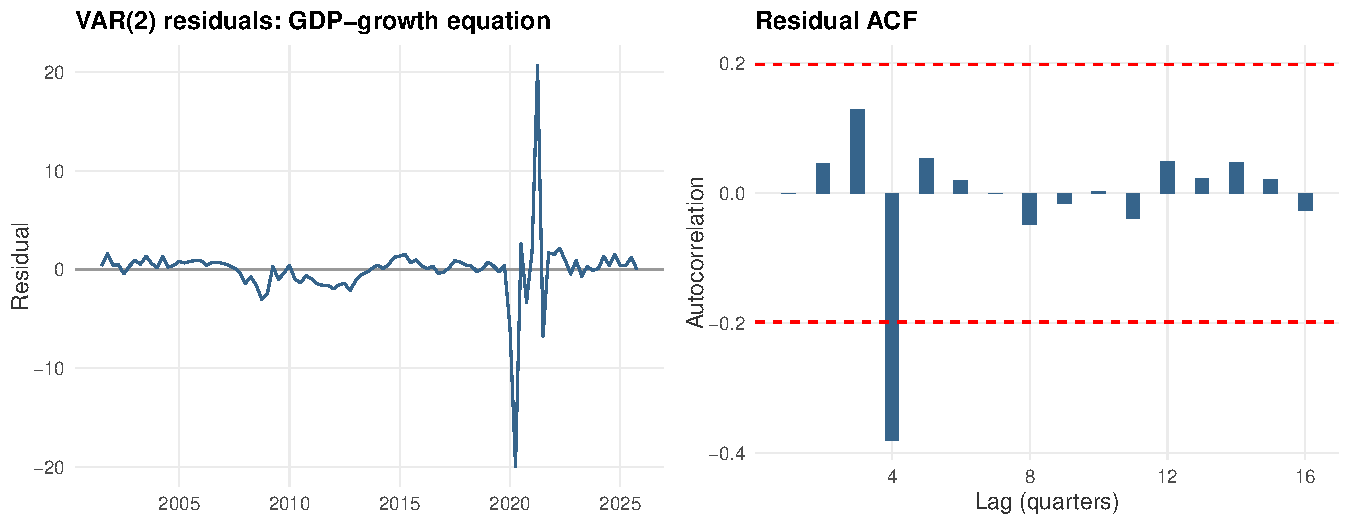
\includegraphics[width=\linewidth]{figures_q/residual_plot.pdf}
    
    {\fontsize{4.8}{5.3}\selectfont
    \setlength{\tabcolsep}{1.2pt}
    \setlength{\abovecaptionskip}{1pt}
    \setlength{\belowcaptionskip}{1pt}
    \begin{table}

\caption{\label{tab:diagnostics}VAR(2) residual diagnostics (quarterly)}
\centering
\begin{tabular}[t]{lrrl}
\toprule
Test & Statistic & p-value & H0\\
\midrule
Portmanteau (residual autocorrelation) & 132.077 & 0.003 & No serial correlation up to lag 12\\
Jarque--Bera (normality, multivariate) & 4140.720 & 0.000 & Normal residuals\\
Multivariate ARCH (heteroskedasticity) & 280.482 & 0.000 & No ARCH effects up to lag 4\\
\bottomrule
\end{tabular}
\end{table}

    }
  \end{column}

  \begin{column}{0.45\textwidth}
    \scriptsize
    The VAR(2) residual diagnostics all reject their nulls: the \textbf{Portmanteau} test finds residual autocorrelation (p $=$ 0.003), \textbf{Jarque--Bera} rejects normality (heavy tails from the COVID-19 outlier), and the multivariate \textbf{ARCH} test detects conditional heteroskedasticity (p $<$ 0.001). These rejections are driven overwhelmingly by the 2020 observations; they caution against an asymptotic reading of the VAR(2) and foreshadow its weak out-of-sample performance, though point-forecast consistency is not destroyed.

    {\fontsize{5}{5.5}\selectfont
    \setlength{\tabcolsep}{1.5pt}
    \setlength{\abovecaptionskip}{1pt}
    \setlength{\belowcaptionskip}{1pt}
    \begin{table}

\caption{\label{tab:stability}Moduli of the companion-matrix roots (quarterly)}
\centering
\begin{tabular}[t]{rr}
\toprule
Root & Modulus\\
\midrule
1 & 0.8225\\
2 & 0.8225\\
3 & 0.6961\\
4 & 0.6961\\
5 & 0.3503\\
\addlinespace
6 & 0.0512\\
\bottomrule
\end{tabular}
\end{table}

    }
    \vspace{0.05cm}
    \scriptsize All roots lie strictly inside the unit circle: the VAR(2) is covariance-stationary.

    \vspace{0.15cm}
  \end{column}
\end{columns}

\end{frame}


% ============================================================
% SLIDE 13: Economic Hypotheses: Granger Causality & IRFs
% ============================================================
\begin{frame}{Economic Hypotheses: Granger Causality \& Impulse Responses}
\label{slide:granger-irf}
\footnotesize

\begin{columns}
  \begin{column}{0.55\textwidth}
    {\fontsize{5.5}{6}\selectfont
    \setlength{\tabcolsep}{2.5pt}
    \setlength{\abovecaptionskip}{2pt}
    \setlength{\belowcaptionskip}{1pt}
    \begin{table}

\caption{\label{tab:granger}Block Granger-causality tests (quarterly)}
\centering
\begin{tabular}[t]{lrr}
\toprule
Null hypothesis & F-statistic & p-value\\
\midrule
Interest rate does not Granger-cause (GDP, infl) & 0.258 & 0.904\\
Inflation does not Granger-cause (GDP, rate) & 2.232 & 0.066\\
GDP growth does not Granger-cause (infl, rate) & 0.556 & 0.694\\
\bottomrule
\end{tabular}
\end{table}

    }
    \scriptsize
    Block Granger causality tests probe predictive relationships. The short-term rate does \emph{not} Granger-cause the (GDP, inflation) block (p $\approx$ 0.90), and growth does not cause the nominal block (p $\approx$ 0.69); only inflation shows marginal predictive content for the others (p $\approx$ 0.07). The multivariate linkages are therefore weak in this sample---consistent with the limited out-of-sample gains from the VAR/BVAR.
  \end{column}

  \begin{column}{0.45\textwidth}
    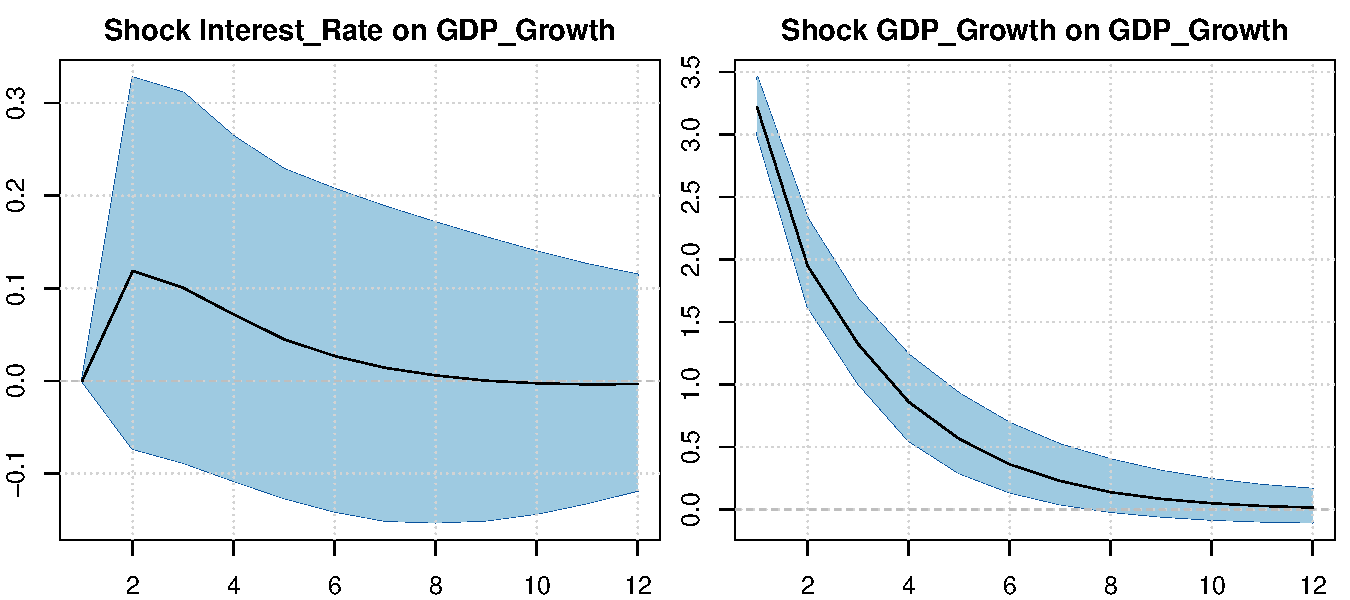
\includegraphics[width=\linewidth]{figures_q/bvar_irf.pdf}
    \scriptsize
    BVAR(2) impulse responses over a 12-quarter horizon. The GDP-growth response to a 1\,$\sigma$ short-rate shock is small and statistically indistinguishable from zero (the 90\% band spans zero at every horizon), so no robust transmission is identified. The own-shock response decays smoothly toward zero, reflecting the stationary autoregressive dynamics.
  \end{column}
\end{columns}

\end{frame}


% ============================================================
% SLIDE 14: Forecasting Evaluation — Point Forecast
% ============================================================
\subsection{Forecast Evaluation}
\begin{frame}{Recursive forecasts: actual vs models}\label{slide:forecast-eval}
\small

\begin{figure}
  \centering
  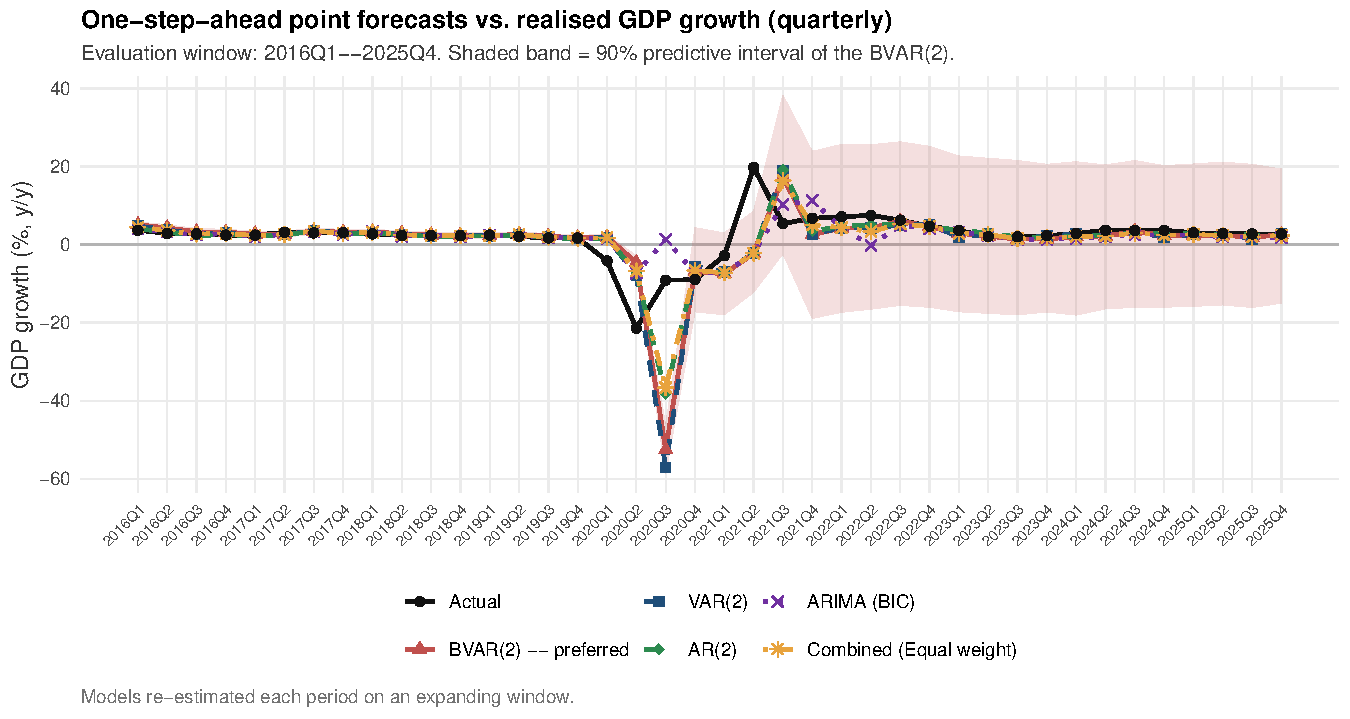
\includegraphics[width=0.72\linewidth]{figures_q/forecast_plot.pdf}
\end{figure}

\vspace{0.05cm}

{\footnotesize
\setlength{\tabcolsep}{4pt}
\begin{table}

\caption{\label{tab:forecast-accuracy}1-step-ahead forecast accuracy (last 10 years, 40 quarters)}
\centering
\begin{tabular}[t]{lrrrr}
\toprule
Model & RMSE & MAE & ME & Theil's U\\
\midrule
ARIMA (BIC) & 4.940 & 2.411 & -0.186 & 0.882\\
Combined (Equal weight) & 6.477 & 2.780 & -0.864 & 1.156\\
AR(2) & 6.736 & 2.788 & -0.810 & 1.203\\
BVAR(2) -- preferred & 8.530 & 3.350 & -1.131 & 1.523\\
VAR(2) & 9.036 & 3.429 & -1.329 & 1.613\\
\bottomrule
\end{tabular}
\end{table}

}

\end{frame}


% ============================================================
% SLIDE 15: Forecast Comparison
% ============================================================
\subsection{Forecast Comparison}
\begin{frame}{Forecast accuracy: ranking and benchmark comparison}\label{slide:forecast-comp}

\small

\begin{columns}
  \begin{column}{0.62\textwidth}
\vspace{-0.2cm}
    {\fontsize{5}{5.5}\selectfont
    \setlength{\tabcolsep}{1.2pt}
    \setlength{\abovecaptionskip}{1pt}
    \setlength{\belowcaptionskip}{1pt}
    \begin{table}

\caption{\label{tab:dm-tests}Diebold--Mariano tests of equal predictive accuracy (squared-loss, quarterly)}
\centering
\begin{tabular}[t]{lrr}
\toprule
Comparison & DM stat & p-value\\
\midrule
BVAR vs VAR(2) & -0.826 & 0.414\\
BVAR vs AR(2) & 1.055 & 0.298\\
BVAR vs ARIMA & 1.087 & 0.284\\
AR(2) vs VAR(2) & -1.000 & 0.323\\
\bottomrule
\end{tabular}
\end{table}

    \vspace{0.1cm}
    \begin{table}

\caption{\label{tab:forecast-coverage}Calibration of one-step-ahead 90\% predictive intervals (quarterly)}
\centering
\begin{tabular}[t]{lrr}
\toprule
Model & Empirical coverage of 90\% PI & Average PI width (pp)\\
\midrule
BVAR(2) -- preferred & 0.850 & 20.171\\
VAR(2) & 0.850 & 6.805\\
AR(2) & 0.850 & 6.738\\
ARIMA (BIC) & 0.850 & 6.803\\
Combined (Equal weight) & 0.875 & 10.129\\
\bottomrule
\end{tabular}
\end{table}

    }

    \vspace{0.5cm}
    \scriptsize \textbf{Cross-frequency check.} At \emph{annual} frequency (1960--2025, 10-year window), where COVID enters as a single annual observation rather than a $-21.5\%$ quarterly crash, the multivariate BVAR(2) is comparatively much stronger. The contrast shows that the quarterly ranking here is driven by the 2020 quarters in the evaluation window, which disproportionately penalise the richer models. \textbf{Note}: the annual analysis lives in a separate \texttt{.qmd} that replicates the same procedures.
  \end{column}

  \begin{column}{0.38\textwidth}
    \tiny
    \begin{itemize}\setlength{\itemsep}{0pt}\setlength{\parskip}{0pt}
      \item \textbf{Point accuracy.} Over the 40-quarter (10-year) window the parsimonious \textbf{ARIMA} forecasts best---the only model to beat a random walk (Theil's $U<1$)---followed by the equal-weight \textbf{Combined} forecast. The richer \textbf{VAR(2)} and \textbf{BVAR(2)} rank last, heavily penalised by the 2020 COVID quarters inside the evaluation window.

      \item \textbf{Statistical significance.} No pairwise Diebold--Mariano test rejects equal predictive accuracy ($p>0.28$ throughout): with 40 one-quarter forecasts and a few extreme COVID losses inflating the loss variance, the differences are not statistically decisive.

      \item \textbf{Interval calibration.} Empirical coverage is similar across models ($\approx$0.85), but the BVAR(2) attains it only with much wider intervals. \textbf{No single model dominates:} ARIMA and the combination are most accurate, while the BVAR(2)---our \emph{a-priori} multivariate benchmark---is destabilised by the COVID observations, echoing Lenza--Primiceri (2022) and Carriero et al.\ (2024) on BVARs after March 2020.
    \end{itemize}
  \end{column}
  
\end{columns}

\end{frame}

\begin{frame}{Conclusions, references, and LLM declaration}
\label{slide:conclusion}
\label{slide:refs}
\scriptsize

\begin{block}{Main conclusions}
\begin{itemize}\setlength{\itemsep}{1pt}\setlength{\parskip}{0pt}
  \item Spain's GDP growth exhibits strong short-run persistence, but is heavily disrupted by the COVID-19 shock.
  \item Adding inflation and the short-term rate does \emph{not} improve out-of-sample accuracy: the multivariate VAR/BVAR are destabilised by COVID (only inflation is a marginal in-sample Granger predictor).
  \item Over the required 10-year window (which contains the COVID-19 crash), the parsimonious \textbf{ARIMA} and the equal-weight \textbf{combination} forecast most accurately; the VAR(2) and BVAR(2) lag, penalised by the 2020 outliers.
  \item \textbf{Caveat:} no Diebold--Mariano test rejects equal accuracy (the ranking is suggestive); excluding COVID the five models are near-tied (RMSE 4.2--4.5), and the VAR(2) residuals reject normality, no-autocorrelation and no-ARCH---cautioning against an asymptotic reading.
\end{itemize}
\end{block}

\textbf{References}
\begin{itemize}\setlength{\itemsep}{1pt}\setlength{\parskip}{0pt}
    \item Bańbura, M., Giannone, D., \& Reichlin, L. (2010). Large Bayesian vector autoregressions. \textit{Journal of Applied Econometrics}, 25(1), 71--92.
    
    \item Litterman, R. B. (1986). Forecasting with Bayesian vector autoregressions - five years of experience. \textit{Journal of Business \& Economic Statistics}, 4(1), 25--38.
    
    \item Barigozzi, M., Lissona, C., \& Tonni, L. (2025). Large datasets for the Euro Area and its member countries and the dynamic effects of the common monetary policy. \textit{arXiv preprint} arXiv:2410.05082v2.
    
    \item Lenza, M., \& Primiceri, G. E. (2022). How to estimate a vector autoregression after March 2020. \textit{Journal of Applied Econometrics}, 37(4), 688--699.

    \item Carriero, A., Clark, T. E., Marcellino, M., \& Mertens, E. (2024). Addressing COVID-19 outliers in BVARs with stochastic volatility. \textit{The Review of Economics and Statistics}, 106(5), 1403--1417.

\end{itemize}

\vspace{0.1cm}

\textbf{AI Disclaimer}: we declare we have employed a number of models, namely Claude Opus 4.7, Sonnet 4.6, and OpenAI ChatGPT for the following purposes: (i) drafting and revising the prose of this report; (ii) suggesting the sequence of diagnostic and forecasting checks; and (iii) refactoring R code for clarity. All modelling choices, parameter interpretations, and substantive conclusions were decided and written by the authors.

\end{frame}

\end{document}